\documentclass[12pt]{article}
\usepackage{amsfonts,amssymb,amsmath}
\usepackage{graphicx}
%\documentstyle[12pt,amsfonts]{article}
%\documentstyle{article}

\setlength{\topmargin}{-.5in}
\setlength{\oddsidemargin}{0 in}
\setlength{\evensidemargin}{0 in}
\setlength{\textwidth}{6.5truein}
\setlength{\textheight}{8.5truein}
%\input ../basicmath/basicmathmac.tex
%
%\input ../lamacb.tex
\input ../CIS515_Project1/mac.tex
\input ../CIS515_Project1/mathmac.tex

\def\fseq#1#2{(#1_{#2})_{#2\geq 1}}
\def\fsseq#1#2#3{(#1_{#3(#2)})_{#2\geq 1}}
\def\qleq{\sqsubseteq}

%
\begin{document}
\begin{center}
\fbox{{\Large\bf Fall 2016 \hspace*{0.4cm} CIS 515}}\\
\vspace{1cm}
{\Large\bf Fundamentals of Linear Algebra and Optimization\\
Jean Gallier \\
\vspace{0.5cm}
Project 1}\\[10pt]
\end{center}

\noindent {\large Problem 1 Part 1}\\
\vspace {0.25cm}\noindent
{\bf Adapt N=5 Case} \\

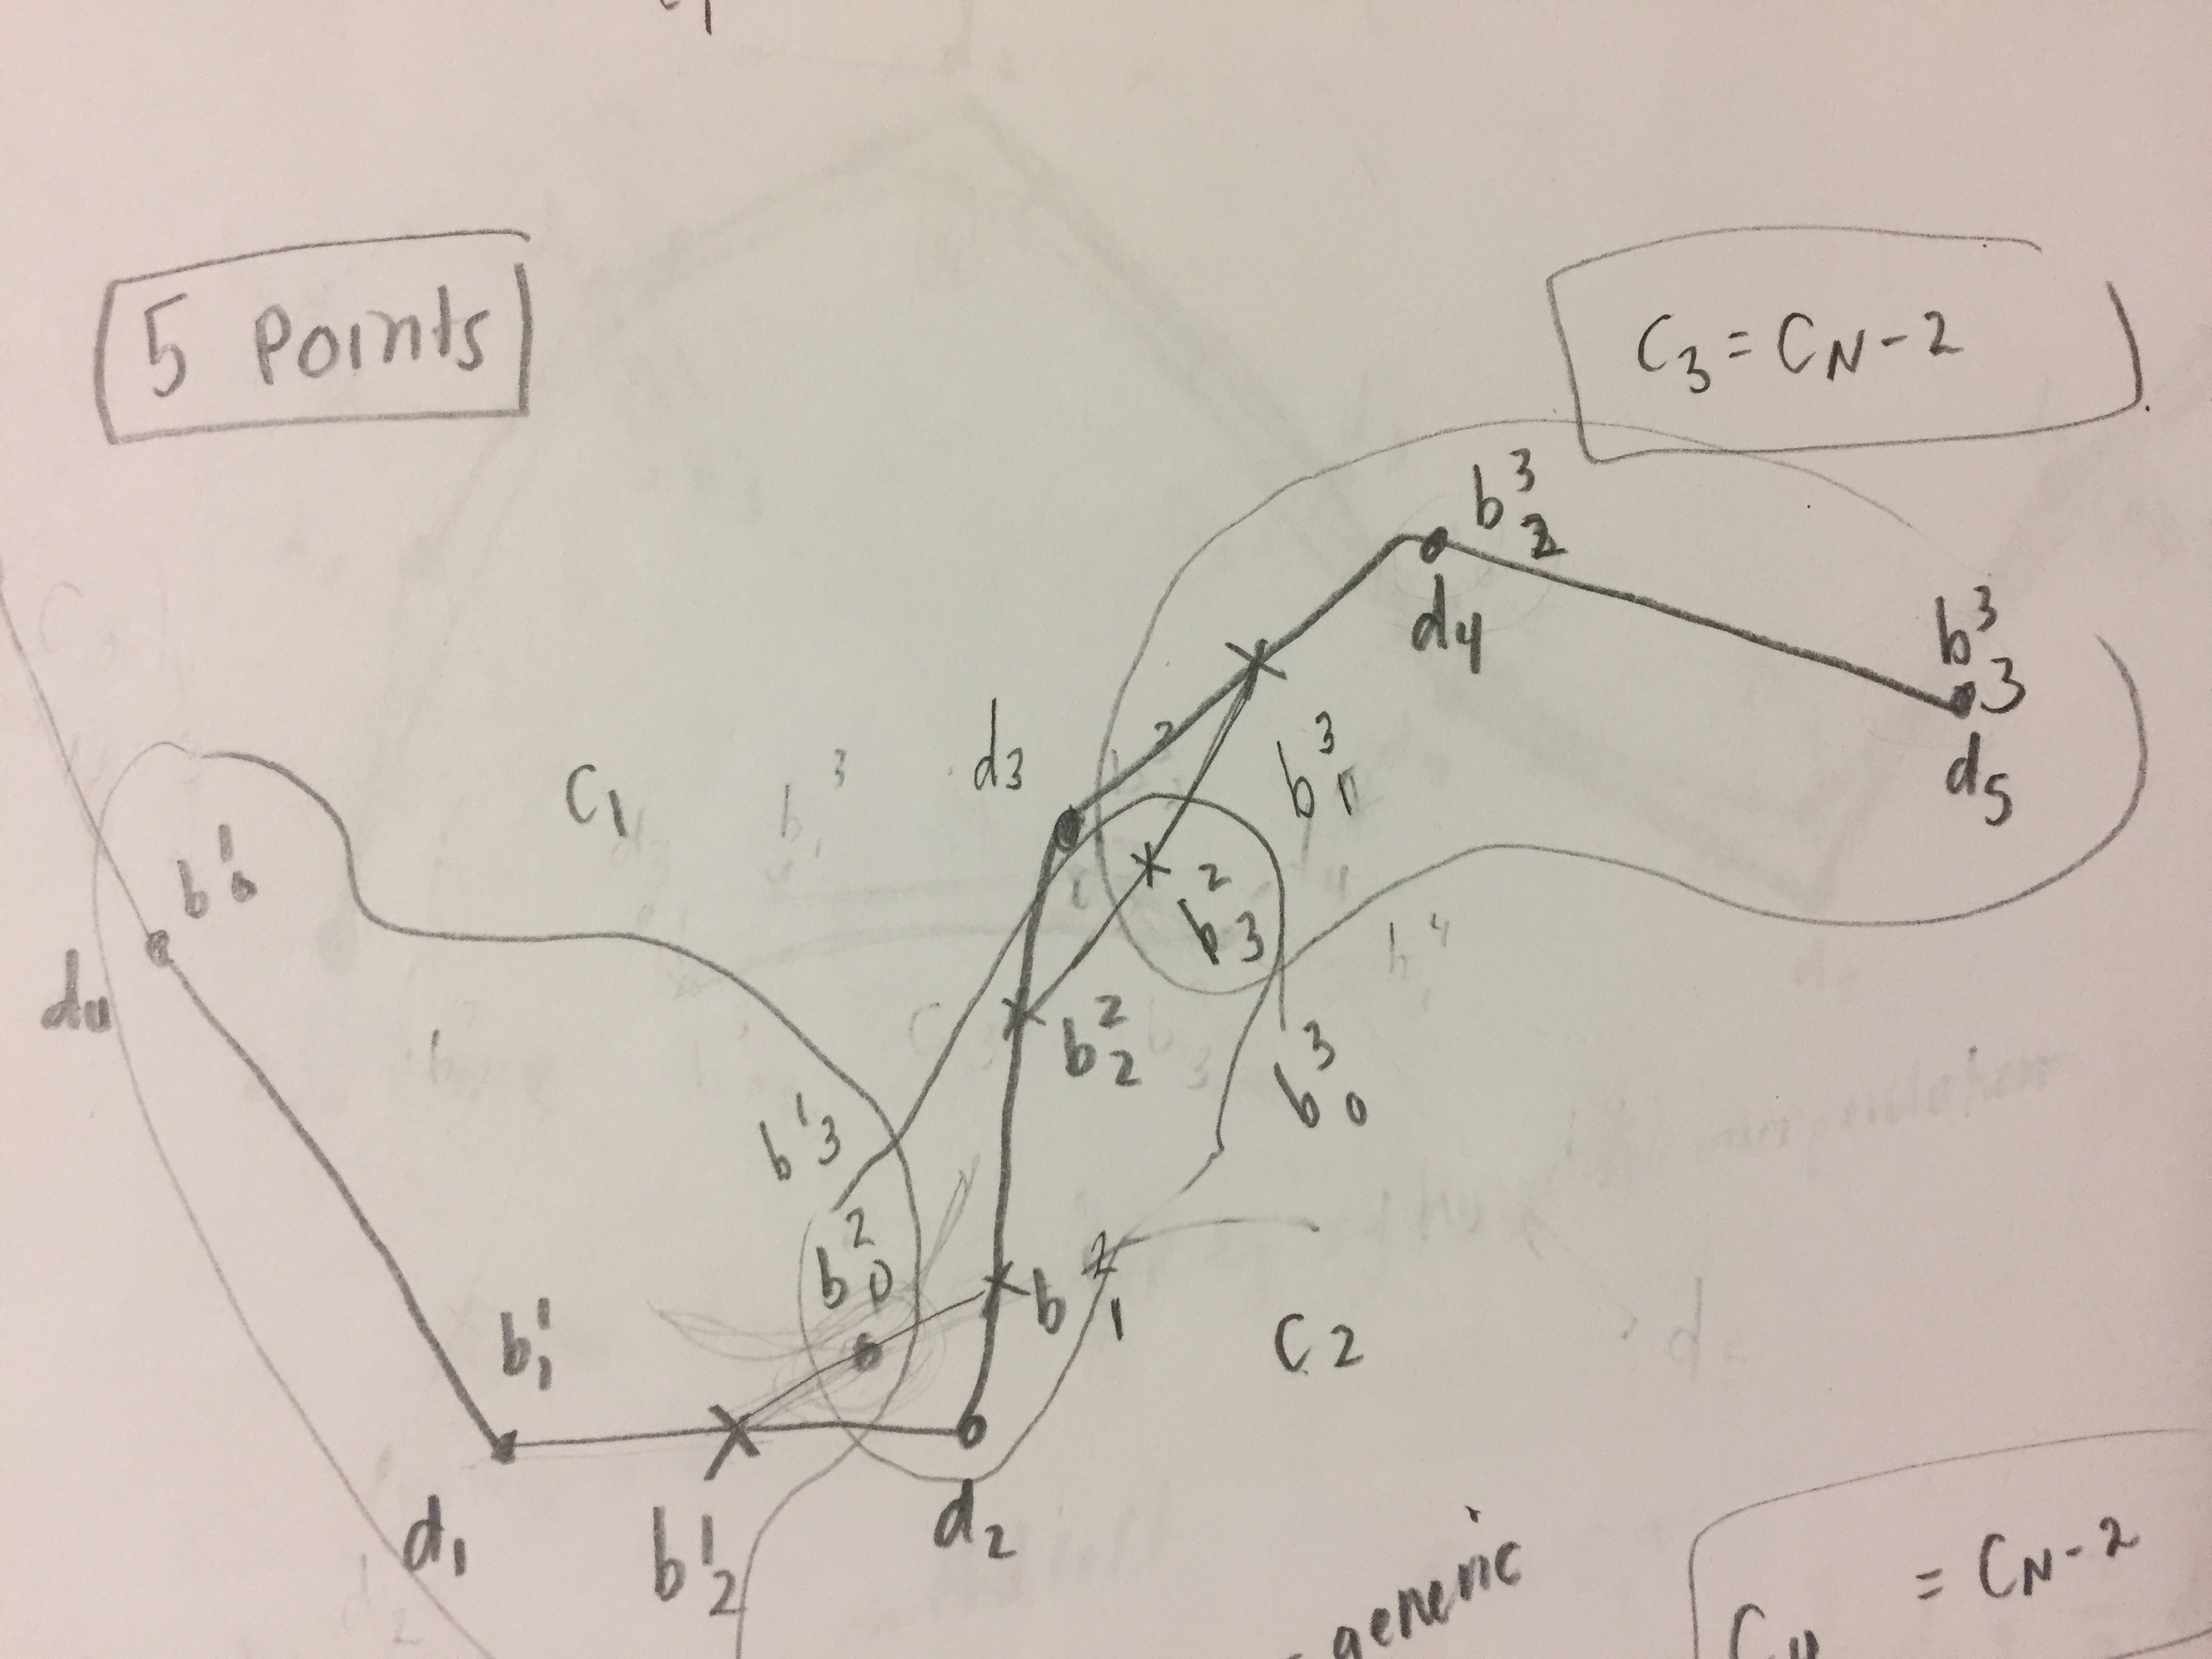
\includegraphics[scale=.1]{5Points}

(C1)
\begin{align*}
b^{1}_{0} =&\; d_0 \\
b^{1}_{1} =&\; d_1 \\
b^{1}_{2} =&\; \frac{1}{2} d_1 + \frac{1}{2}d_2 \\
b^{1}_{3} =&\; \frac{1}{4} b^{1}{2} + \frac{1}{2} b^{2}_{1} =\frac{1}{4}d_1 +\frac{7}{12}d_2 + \frac{1}{6}d_3 \\
\end{align*}

(C2)
\begin{align*}
b^{2}_{0} =&\; \frac{1}{2} b^{1}_{2} + \frac{1}{2} b^{2}_{1}\\
=&\; \frac{1}{4} d_1 + +\frac{7}{12}d_2 + \frac{1}{6}d_3 \\
b^{2}_{1} =&\; \frac{2}{3} d_2 + \frac{1}{3}d_3 \\
b^{2}_{2} =&\; \frac{1}{3} d_2 + \frac{2}{3}d_3 \\
b^{2}_{3} =&\; \frac{1}{2} b^{2}{2} + \frac{1}{2} b^{3}_{1} =\frac{1}{6}d_2 +\frac{4}{6}d_3 + \frac{1}{6}d_4 \\
\end{align*}

(C3)
\begin{align*}
b^{3}_{0} =&\; \frac{1}{2} b^{2}{2} + \frac{1}{2} b^{3}_{1} =\frac{1}{6}d_2 +\frac{4}{6}d_3 + \frac{1}{6}d_4 \\
b^{3}_{1} =&\; \frac{1}{2}d_3 + \frac{1}{2} d_4 \\
b^{3}_{2} =&\; d_4 \\
b^{3}_{3} =&\; d_5 \\
\end{align*}

\vspace {0.25cm}\noindent
{\bf Adapt N=6 Case} \\

\includegraphics[scale=.1]{6Points}

(C1)
\begin{align*}
b^{1}_{0} =&\; d_0 \\
b^{1}_{1} =&\; d_1 \\
b^{1}_{2} =&\; \frac{1}{2} d_1 + \frac{1}{2}d_2 \\
b^{1}_{3} =&\; \frac{1}{4} b^{1}{2} + \frac{1}{2} b^{2}_{1} =\frac{1}{4}d_1 +\frac{7}{12}d_2 + \frac{1}{6}d_3 \\
\end{align*}

(C2)
\begin{align*}
b^{2}_{0} =&\; \frac{1}{2} b^{1}_{2} + \frac{1}{2} b^{2}_{1}\\
=&\; \frac{1}{4} d_1 + +\frac{7}{12}d_2 + \frac{1}{6}d_3 \\
b^{2}_{1} =&\; \frac{2}{3} d_2 + \frac{1}{3}d_3 \\
b^{2}_{2} =&\; \frac{1}{3} d_2 + \frac{2}{3}d_3 \\
b^{2}_{3} =&\; \frac{1}{2} b^{2}{2} + \frac{1}{2} b^{3}_{1} =\frac{1}{6}d_2 +\frac{4}{6}d_3 + \frac{1}{6}d_4 \\
\end{align*}

(C3)
\begin{align*}
b^{3}_{0} =&\; \frac{1}{2} b^{2}{2} + \frac{1}{2} b^{3}_{1} =\frac{1}{6}d_2 +\frac{4}{6}d_3 + \frac{1}{6}d_4 \\
b^{3}_{1} =&\; \frac{2}{3}d_3 + \frac{1}{1} d_4 \\
b^{3}_{2} =&\; \frac{1}{3}d_3 + \frac{2}{3} d_4 \\
b^{3}_{3} =&\; \frac{1}{2} b^{3}_{2} + \frac{1}{2}b^{1}_{4} = \frac{1}{6} d^{3} + \frac{7}{12} d_4 + \frac{1}{4} d_5\\
\end{align*}

(C4)
\begin{align*}
b^{4}_{0} =&\; \frac{1}{2} b^{3}_{2} + \frac{1}{2}b^{1}_{4} = \frac{1}{6} d^{3} + \frac{7}{12} d_4 + \frac{1}{4} d_5\\
b^{4}_{1} =&\; \frac{1}{2}d_4 + \frac{1}{2} d_5 \\
b^{4}_{2} =&\; d_5 \\
b^{4}_{3} =&\; d_6 \\
\end{align*}



\vspace {0.25cm}\noindent
{\bf Adapt N=4 Case Not yet updated} \\

(C1)
\begin{align*}
b^{1}_{0} =&\; d_0 \\
b^{1}_{1} =&\; d_1 \\
b^{1}_{2} =&\; \frac{1}{2} d_1 + \frac{1}{2}d_2 \\
b^{1}_{3} =&\; \frac{1}{4} b^{1}{2} + \frac{1}{2} b^{2}_{1} =\frac{1}{4}d_1 +\frac{7}{12}d_2 + \frac{1}{6}d_3 \\
\end{align*}

(C2)
\begin{align*}
b^{2}_{0} =&\; \frac{1}{2} b^{1}_{2} + \frac{1}{2} b^{2}_{1}\\
=&\; \frac{1}{4} d_1 + +\frac{7}{12}d_2 + \frac{1}{6}d_3 \\
b^{2}_{1} =&\; \frac{2}{3} d_2 + \frac{1}{3}d_3 \\
b^{2}_{2} =&\; \frac{1}{3} d_2 + \frac{2}{3}d_3 \\
b^{2}_{3} =&\; \frac{1}{2} b^{2}{2} + \frac{1}{2} b^{3}_{1} =\frac{1}{6}d_2 +\frac{4}{6}d_3 + \frac{1}{6}d_4 \\
\end{align*}

\noindent {\large Problem 1 Part 2}\\

The indices in the interpolation problem defined in the notes and slides are expressed in the form $d_{-1}$. Thus the indices in the project for Problem 1 are off by 1. The points $d_1$ to $d_{N-1}$ are the control points on the Bezier cubic segments, and points $d_{-1}$ and $d_{N}$ are the first and last point de Boor control points respectively. Each of the $x_i = b^{i}_{3}$. \\

The first point, $d_1$, can be written in the form, 
\begin{align*}
x_1 =&\; b^{1}_{3} \\
x_1  =&\; \frac{1}{4}d_0 +\frac{7}{12}d_1 + \frac{1}{6}d_2 \\
6(x_1  =&\; \frac{1}{4}d_0 +\frac{7}{12}d_1 + \frac{1}{6}d_2) \\
6x_1  =&\;  \frac{3}{2}d_0 +\frac{7}{2}d_1 + d_2 \\
6x_1  - \frac{3}{2}d_0  =&\; \frac{7}{2}d_1 + d_2 \\
\end{align*}

The second point, $d_2$, can be written in the form,
\begin{align*}
x_2 =&\; b^{2}_{3} \\
x_2  =&\; \frac{1}{6}d_1 +\frac{4}{6}d_2 + \frac{1}{6}d_3 \\
6(x_2  =&\; \frac{1}{6}d_1 +\frac{4}{6}d_2 + \frac{1}{6}d_3 \\
6x_2  =&\;  d_1 + 4d_2 + d_3 \\
\end{align*}

The last two points, $d_{N-2}$ and $d_{N-1}$ are the first two points in the Bezier cubic segments, not the last. Now $x_{N-2}$ and $x_{N-1}$ are equal to $b^{N-2}_{0}$ and $b^{N-1}_{0}$ respectively.\\

The second to last point, $d_{N-2}$, can be written in the form, 
\begin{align*}
x_{N-2} =&\; b^{N-2}_{0} \\
x_{N-2} =&\; \frac{1}{6}d_{N-3} +\frac{4}{6}d_{N-2} + \frac{1}{6}d_{N-1} \\
6(x_{N-2} =&\; \frac{1}{6}d_{N-3} +\frac{4}{6}d_{N-2} + \frac{1}{6}d_{N-1}) \\
6x_{N-2} =&\; d_{N-3} + 4d_{N-2} + d_{N-1} \\
\end{align*}

The last point, $d_{N-1}$, can be written in the form, 
\begin{align*}
x_{N-1} =&\; b^{N-1}_{0} \\
x_{N-1} =&\; \frac{1}{6}d_{N-2}+\frac{7}{12}d_{N-1} + \frac{1}{4}d_N \\
6(x_{N-1} =&\; \frac{1}{6}d_{N-2}+\frac{7}{12}d_{N-1} + \frac{1}{4}d_N) \\
6x_{N-1} =&\; d_{N-2}+\frac{7}{2}d_{N-1} + \frac{3}{2}d_N \\
6x_{N-1} - \frac{3}{2}d_N =&\; d_{N-2}+\frac{7}{2}d_{N-1} \\
\end{align*}
\end{document}